\chapter{Architectuur}\label{ch:functioneel-ontwerp} % Chapter title

Om SOUP-analyses periodiek en geautomatiseerd uit te kunnen voeren moet er een systeem worden ontworpen dat op verschillende plekken binnen de dev-stack van Eaglescience opereert. Bij het ontwerp wordt er rekening gehouden met de resultaten uit het onderzoek en de requirements die in het vorige hoofdstuk uitgewerkt zijn.


De SOUP module moet op twee manieren geautomatiseerd analyses uit kunnen voeren. Ten eerste op het moment dat er een build wordt gestart mag er aangenomen worden dat er veranderdingen zijn in de source code met daarbij potentieel veranderingen in dependencies. De Jenkins pipeline zal als dit is gebeurt een update geven in de vorm van nieuwe informatie. De method hiervoor wordt hieronder verder beschreven in de sectie over Jenkins. Ten tweede moeten er periodiek automatisch analyses worden uitgevoerd op projecten waar al informatie over bekend is bij de SOUP module. Hiervoor dient een eigen methode te worden gezocht die zelf een omgeving kan opzetten waar vervolgens analyses uitgevoerd kunnen worden ook hier wordt later een sectie aan geweid.

De informatie die beschikbaar is moet vervolgens worden weergeven in de portal die al bestaat binnen Eaglescience. Hiervoor dient er een module worden toegevoegt aan de bestaande portal samengevat dienen er dus de volgende onderdelen te worden ontwikkeld:

\begin{enumerate}
    \item \textbf{SOUPAPI}: De API is verantwoordelijk voor een aantal zaken binnen het systeem. Ten eerste moet het de rauwe informatie verkrgen uit de buildstraat omzetten in een uniform datamodel. Welke vervolgens kan worden gebruikt om middels een webapplicatie de relevantie informatie te serveren.
    \item \textbf{Jenkins build Pipeline}: Verkrijgen van informatie over eventueel gevonden kwetsbaarhden, als ook meta data over de gebouwden en/of uitgerolde projcten.
    \item \textbf{Analyse Container omgeving}: Een omgeving waarin SBT en NPM projecten kunnen worden gebouwd waarop een analyse uitgevoerd kan worden door de SOUP API. de informatie die hier uit voor komt is voor de SOUP Module om inzichten te genereren voor de gebruiker.
    \item \textbf{Portal}: De Portal is de interface die het mogelijk maakt om interactie te verkrijgen met SOUP API. Interactie in de vorm van het opvragen van de gewenste informatie als ook instellingen waarbij de werking van de API kan worden beinvloed.
\end{enumerate}
Dit hoofdstuk zal de architectuur van deze hoofddelen als ook de relatie tot elkaar toelichten.


\section{Architectuur ontwerp}\label{sec:architectuur-ontwerp}
In figuur~\ref{fig:UML-ComponentDiagram} zijn de drie hoofdonderdelen getoont met daarbij de relatie die elk onderdeel met elkaar heeft.

Als we van boven naar beneden door het figuur lopen komen we eerst de Jenkins buildstraat tegen. De integratie met Jenkins is benodigd om bij een door een ontwikkelaar gestarte build of uitrol een analyse te doen op een project. Naast de analyse worden de nieuwste versies van de declaraties als ook project meta data verstuurt. Op deze manier weet de SOUP API de laatst gescannde versie van het project. Het datapakket dat wordt verstuurd is een combinatie van de raporten gegenereerd door de SLA tool, een timestamp, en data over het project(naam, commitHash, datum van de scan etc.)

Deze Data wordt door de ReportParserModule in de SOUP API ontleed in de raporten, en de data over het project. De rapporten worden geconverteerd in een datamodel waarin alleen de gewenste data wordt opgeslagen.(uit eerste blikken op de rapporten bestaan deze uit veel informatie die niet gewenst is voor deze toepassing, hier is echter in later stadium zeker verder onderzoek voor nodig.) De data over de projecten bevatten naast de metadata over het project en de scan ook de dependency declaraties van de modules. deze dienen ook te worden opgeslagen voor het mogelijkmaken van de periodieke scans. De SOUP API omvat ook een controller, een module dat zorgdraagd voor de functionaliteiten van de API zoals schrijven en lezen van de database. Maar ook enkele mechanieken die het mogelijk maken om een periodieke analyse uit te kunnen voeren. Enkele belangrijke zijn,
ScanTrigger geeft de mogelijkheid om een al bekende projecten on-demand te scannen.
ScanQ is een module  dat zorg draagt voor het bijhouden welke scans er plaats moeten vinden en welke al geweest zijn. De ScanEngine haalt de eerste uit de ScanQ Welke vervolgens de ContainerControl vraagt om een container op te starten met de gegevens die bekend zijn. Op het moment dat de ScanEngine de gegevens in goed orde heeft ontvangen krijgt het de opdracht om de container te vernietigen. DB control zorgt voor CRUD operaties die de modulen binnen de controller nodig heeft.

In de Portal wordt een module toegevoegd welke samenwerkt met de LDAP module voor credentials en rechten/rollen op de verschillende projecten. Er is ook een samenwerking met de projects module om inzicht in een te krijgen in de bestaande projecten. In de komende hoofstukken wordt iedere onderdeel van het systeem verder uitgewerkt.
\begin{figure}
    \myfloatalign
    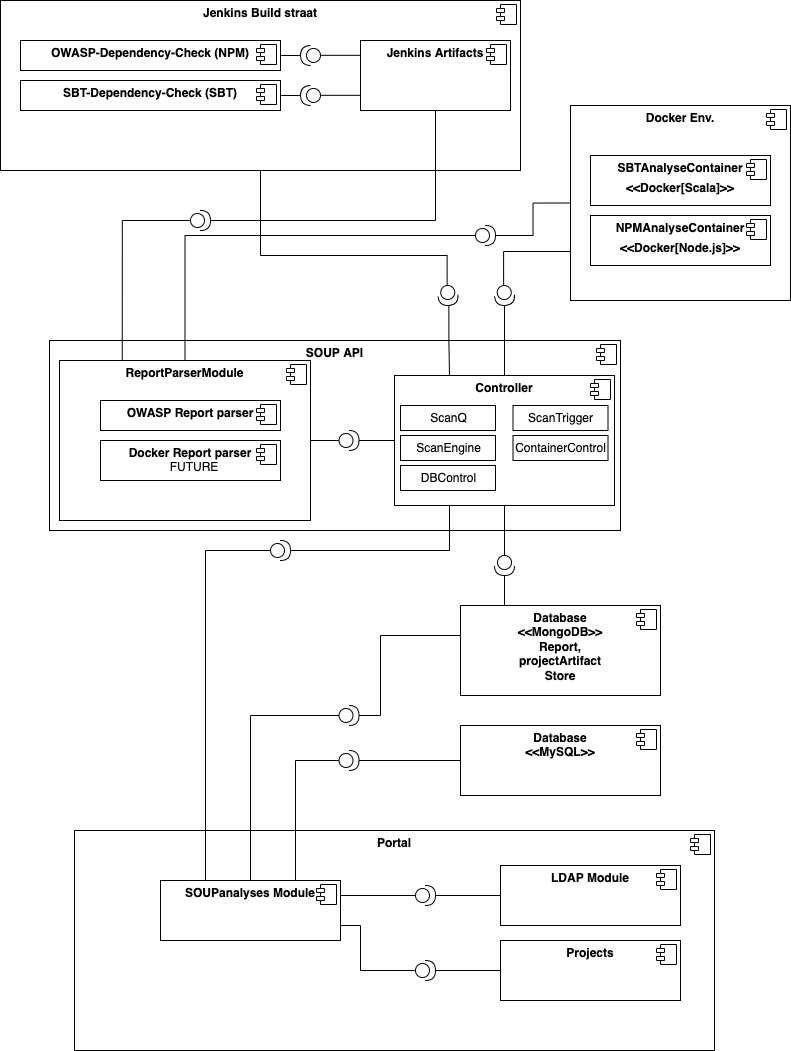
\includegraphics[width=10cm]{gfx/UMLcomponentDiagram}
    \caption{Component diagram}
    \label{fig:UML-ComponentDiagram}
\end{figure}

\section{Integratie Jenkins Buildstraat}\label{sec:integratie-jenkins-buildstraat}
In de jenkins buildstraat moeten enige aanpassingen worden gedaan om ervoor te zorgen dat gegevens vanuit een build worden gestuurd naar de SOUP API. In deze sectie wordt uitgewijd over welke data er moet worden verstuurd en in welke vorm. Als ook de methoden en technieken die moeten worden geimplementeerd om deze data te verkrijgen en vervolgens te versturen.

\subsection{Datamodel}\label{subsec:datamodel}

Om in de portal een overzicht te kunnen weergeven over de analyses die zijn uigevoerd met de daarbij behordende resultaten moet er op een uniforme manier gegevens uit de jenkins straat komen. Naast data over het project.
De data die de Portal minimaal nodig heeft om een overzicht te weer te geven over de stand van zaken over kwetsbaarheden binnen projecten zijn de volgende


Uit de buildstraat komt het volgende datamodel welke gebruikt kan worden door de SOUP API voor verdere verwerking. De data wat verstuurt wordt dient zal in een JSON file worden geupload naar de API.

\begin{lstlisting}[caption={Datamodel vanuit Jenkins},label=lst:DatamodelJenkins]
{
  "projectnaam":"GroeiGids",
  "JenkinsScan": true,
  "BuildHash": "fb5f5cb47bbd0cbf2f4771c55242fedbf41c5efc",
  "buildDate": "22-01-2022",
  "buildModules":["App", "portal","backend"],
  "reports": [
    {
      "NPM-portal-report": {
        "tool": "OWASP-NPM",
        "report": " {<<REPORT>>}
      }
    },
    {
      "NPM-app-Report": {
        "tool": "OWASP-NPM",
        "report": " {<<REPORT>>}
      }
    },
    {
      "sbt-backend-report": {
        "tool": "OWASP-NPM",
        "report": " {<<REPORT>>}
      }
    }
  ],
  "dependencies": [
    {
      "npm-portal-deps": {}
    },
    {
      "npm-app-deps": {}
    },
    {
      "sbt-backend-deps": {}
    }
  ]
}
\end{lstlisting}

\subsection{Architectuur}


eze gegevens moeten in een Datamodel worden verstuurd.

Ook in de projecten die moeten worden gescanned moeten er plugins worden opgegeven die het mogelijk maken om de analyse uit te voeren. In de eerste iteratie van het ontwerp is dit de plugin voor SBT\footnote{https://github.com/albuch/sbt-dependency-check} en NPM\footnote{https://github.com/etnetera/owasp-dependency-check}. Latere iteraties moeten het mogelijk maken om andere platformen te ondersteunen.

Om gegevens die


De integratie dient alleen te worden gebruikt op het moment dat er een nieuwe build gestart is waarbij er potentieel nieuwe informatie over dependencies verwacht kunnen worden.

Als we het sequentie diagram uit figuur~\ref{fig:UML-JenkinsIntegratie} van links naar rechts doorlopen dan zien we dat een build getriggered wordt op de normale manier hier zullen dan geen aanpassingen worden gedaan.
In de buildtest stap wordt een container opgestart waarin het project wordt gebuild. Dit is het moment dat de SBT SOUP-analyse plugin een analyse uit kan voeren. De output van deze analyse moet worden opgeslagen in Artifacts van de build onder de volgende naam [PLATFORM]-[MODULE]-report.json. Aan het einde van deze stap

In de postbuild stap moet er op het moment dat er een success is alle reports, dependency informatie en project meta data worden samengevoegd en worden verstuurt naar de SOUP API die de gegevens verder verwerkt.


\begin{figure}
    \myfloatalign
    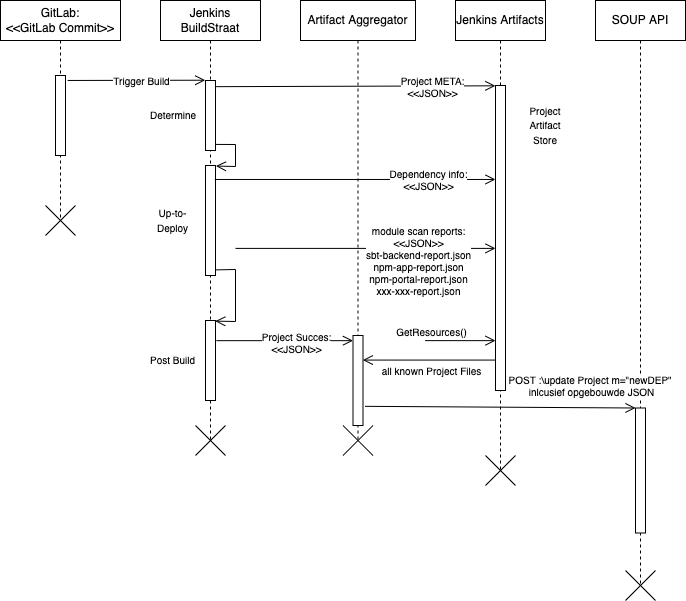
\includegraphics[width=10cm]{gfx/UMLJenkinsIntegratie}
    \caption{Sequence Diagram Jenkins > SOUP API}
    \label{fig:UML-JenkinsIntegratie}
\end{figure}

Het is mogelijk om middels de Jenkins API artifacts te downloaden .... > https://stackoverflow.com/questions/35920756/is-there-any-jenkins-api-to-get-artifacts-name-and-download-it



Voor iedere uitbreiding van omgeving moet een SCA tool worden gevonden die op een gestructureerd manier data aan kan leveren aan de SOUP API.


%https://github.com/etnetera/owasp-dependency-check for Node.js /NPM
%https://github.com/albuch/sbt-dependency-check for SBT
%
%https://github.com/eliasgranderubio/dagda niet zelfde als OWASP maar wellicht usefull


\section{SOUP API}

De SOUIP API is een omgeving welke verantwoordelijk is voor de werking van de soup module. De werking is opgedeeld in twee hoofdmodulen, een ReportParser wat is opgezet om Raporten van verschillende tooling om te zetten naar het datamodel dat gehanteerd wordt binnen de portal applicatie. Deze parser is nodig om de enorme hoeveelheid data die uit de analyses komt te filteren. De opzet is zo gekozen om er voor te zorgen dat er zonder veel moeite een parser kan worden toegevoegd die in staat is om rapporten van andere platformen om te zetten naar het interne datamodel. De controller is voornamelijk verantwoordelijk voor de periodieke analyses die op voor de SOUP API bekende projecten wordt gedaan. In onderstaande secties wordt de werking en relaties met elkaar verder uigewerkt.

\subsection{SOUPAPI Controller}
De controller is verantwoordelijk voor het orchestreren van periodieke scans die gedaan moeten worden op voor de SOUP API Bekende\footnote{De SOUP API weet van projecten op het moment dat er een project is aangemaakt via de portal en er een build is geweest van ditzelfde project met daarin de in de vorige sectie beschreven module.} projecten. Het omvat een aantal features zoals een scheduler die de projecten op basis van ingestelde tijd aanbied aan de analyser die de analyses uitvoerd.

\subsection{SOUPAPI Report Parser}
De reportParser is een API met daarin een aantal methoden specifiek geschreven voor de binnenkomende rapporten in dit onwerp komt een parser voor het OWASP rapport dat gegenereerd wordt door zowel de SBT als NPM SCA tools die eerder geselecteerd zijn.
